\documentclass[11pt]{report}

\usepackage{graphicx}
\usepackage{float}
\usepackage[utf8]{inputenc}
\usepackage{graphicx}
\usepackage{graphics}
%\usepackage{pifont}
\usepackage{color}
\usepackage{subfigure}



%\usepackage{xcolor}
\usepackage[table]{xcolor}
%\definecolor{silver}{RGB}{192,192,192}
%\usepackage[margin=1in]{geometry}
\usepackage{float}
%\usepackage{enumitem}
\usepackage{etoolbox}
\usepackage{lipsum}
\usepackage{setspace}
\usepackage{titlesec}
\usepackage{subfig}
%\usepackage[per-mode=fraction]{siunitx}
%\usepackage{numprint}
%\usepackage{array}
%\usepackage{sidecap}
%\usepackage{wrapfig}

%Justify 
\usepackage{amsmath}
%\usepackage{amssymb}
%\usepackage{mathrsfs}
%\usepackage{mathtools}

\usepackage[french]{babel}
%\frenchbsetup{StandardLists=true} %alignement
%\definecolor{silver}{RGB}{192,192,192}
%\usepackage{hyperref}
%\usepackage[nottoc]{tocbibind}

\usepackage{amsmath}  %pour les matrices

\usepackage[squaren, Gray, cdot]{SIunits} %Symboles

\usepackage[a4paper,top=3cm,bottom=2cm,left=3cm,right=3cm,marginparwidth=1.75cm]{geometry}



  
\titleformat{\chapter}[display]
 {\normalfont\huge\bfseries\filcenter}{\chaptertitlename\ \thechapter}{16pt}{\Huge}
  
%\subsubsectionfont{\normalfont\large\itshape\underline}

\begin{document}

\newcommand{\HRule}{\rule{\linewidth}{0.5mm}}

\begin{minipage}{0.47\textwidth} \begin{flushleft}
		
\includegraphics[scale =0.3]{images/logo_snep.png}
\end{flushleft}\end{minipage}
\begin{minipage}{0.47\textwidth} \begin{flushright}
		
\includegraphics[scale = 0.3]{images/logo_snep.png}
\end{flushright}\end{minipage} 
\vspace*{-1.5cm}						
\begin{center}
	\textsc{\large 
	\large 	SOCIETE NATIONALE D'ELECTROLYSE\\ \vspace{0.2cm}
\large ET\\ \vspace{0.2cm}
\large PYTROCHIMIE
  }\\[2cm]	
	
	\begin{minipage}{1\textwidth} 
		\begin{center}
			\textsc{\Large \textbf{Rapport du Projet Compound}} \\ [0.3cm]
		\end{center}
	\end{minipage}\\[0.3cm]


	
	
	
	\vspace*{0.5cm}	
	\HRule \\[0.05cm]	
	\begin{center} 
		\LARGE \bfseries{
			Cost effective prediction System
		}\\[0.3cm]
	\end{center}		
	\HRule \\[0.6cm]
	
	\begin{figure}[H]
		\begin{center}
			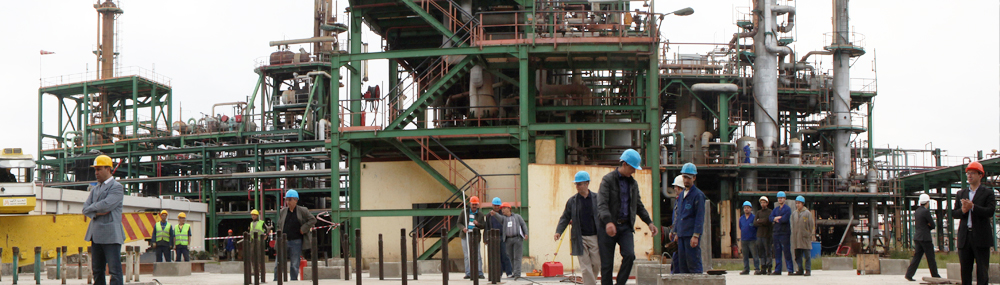
\includegraphics[width=12cm]{images/couvert.jpg}
			\label{fig:figure}
		\end{center}
	\end{figure}

\begin{minipage}{1\textwidth}												

\end{minipage}\\[2cm]
	
	
	\begin{minipage}{1\textwidth}												
		\begin{center}	 \large															
			\emph{Réalisé par:}\\[0.3cm]
			\textbf{ACHAQ Abdelkarim } \\
			\textbf{FILALI Ahmed } \\
		
		\end{center}																		
	\end{minipage}\\[3cm]
	
	
	%\bigskip{}
	\begin{minipage}{1\textwidth}												
		\begin{center}	 \large															
			
			%\includegraphics[scale = 0.6]{} \\
		\end{center}															
	\end{minipage}\\[0.5cm]
		\begin{minipage}{1\textwidth}												
					
	\end{minipage}\\[2cm]
	
	
	\begin{minipage}{1\textwidth}
	\begin{center} \large
		\emph{Encadré par :}\\[0.3cm]

		\centering	\item  \textbf{Mr. CHERKAOUI Mohammed} 
					
	\end{center}
	\end{minipage}\\[2.5cm]
	
\end{center}

\setcounter{page}{0}
\thispagestyle{empty}

\newpage
\newpage
\pagenumbering{roman}



%*********************************************Resume************************************************************
\chapter*{Résumé}
\addcontentsline{toc}{chapter}{\numberline{}Résumé}

Ce document présente de manière synthétique le stage
d'application réalisé au sein de la société Esvitech au cours de
l'été 2018. L'objectif était d’effectuer la détection et la lecture
automatique de plaques d’immatriculation de véhicules
automobiles Marocaines. Pour cela nous avons réalisé un état de
l’art et une étude préalable afin de recueillir les informations
nécessaires pour permettre de cerner les différents traitements à
implémenter dans ce système. Une application portable
interactive a été développée et les résultats ont été très
satisfaisants.
Dans ce système, plusieurs prétraitements de filtrage de bruits,
de transformations d’images et de détection ont été réalisés.
Ensuite, des opérations de segmentation, de détection de
contours et de reconnaissance de forme de caractères ont permis
de répondre aux besoins exigés dans ce projet.
%*********************************************Abstract************************************************************
\chapter*{Abstract}
\addcontentsline{toc}{chapter}{\numberline{}Abstract}
The aim of this project is to carry out the detection and the
automatic reading of license plates of Moroccan motor vehicles.
For this purpose we have carried out a state of the art and a
preliminary study in order to gather the information necessary to
identify the different treatments to be implemented in this
system. An interactive portable application
has been developed and the results have been very satisfactory.
In this system, several pre-treatments of noise filtering, image
transformations and detection have been carried out. Subsequent
segmentation, contour detection and character recognition
operations were carried out to meet the needs of the project.



\tableofcontents
\setcounter{tocdepth}{5}

\newpage
\listoffigures


\newpage
\sf
%-------------------------------------------------------------------------------------------------------------------
%************************************************Intoduction********************************************************
%-------------------------------------------------------------------------------------------------------------------
\chapter*{Introduction}
\addcontentsline{toc}{chapter}{\numberline{}Introduction}
\subsubsection{CONTEXTE}
Le numéro d’immatriculation représente un moyen efficace pour identifier les véhicules. Il
s’agit d’une information unique pour chaque voiture.
Fréquemment, il est nécessaire d’identifier les plaques d’immatriculation des véhicules pour
la sécurité. Les informations extraites peuvent être utilisées pour plusieurs intérêts, comme
le contrôle d’accès et de flux, la surveillance des passages aux frontières et aux péages, la
recherche de véhicules suspects ou encore la lutte contre la criminalité, etc. Ceci rend leurs
lectures cruciale et inévitable dans tous ces domaines.
Dans notre projet, nous nous intéressons à la reconnaissance et la lecture automatique de
plaques d’immatriculation à partir de captures d’images prises sur le devant ou à l’arrière
des véhicules.
\subsubsection{PROBLEMATIQUE ET OBJECTIF}
La vraie problématique pour identifier des plaques d’immatriculation réside dans le
fait de pouvoir faire de la reconnaissance optique de caractères sur une petite partie
d’image extraite de séquences enregistrées, souvent dans des conditions de grande vitesse
et de faible luminosité. De plus, le fait de ne disposer que de très peu d’images hautes
définition par seconde sur la plupart des caméras vidéo entraîne un manque de netteté lors
de la capture de ces images. Pour cela, il faut procéder à un prétraitement de ces images à
la détection des contours, pour permettre une reconnaissance optique assez fiable des
caractères.
Ce que nous visons à travers notre travail est de faciliter la tâche, d'identification des
caractères du matricule en exploitant les avantages que peux offrir le traitement d’image.
Pour cela, nous avons développé une application qui consiste à réaliser des prétraitements,
la détection et la lecture automatique des caractères.
\subsubsection{PLAN DE CE RAPPORT}
Pour cela, nous avons décomposé notre mémoire comme suit :
Le premier chapitre, nous commencerons par définir la lecture automatique de
plaques d’immatriculation.
Après ceci, nous allons présenter les algorithmes qui doivent être réalisés pour quele logiciel puisse identifier une plaque d'immatriculation et les difficultés qui en résultent.
Nous finirons ce chapitre par quelques exemples de systèmes existants.
Dans le deuxième chapitre, nous allons présenter une étude sur le traitement
d’images et les notions de base nécessaires à la compréhension de ces techniques.
Le troisième chapitre, nous avons présenté un certain nombre d'outils que nous
avons utilisés pour réaliser notre travail.
Le quatrième et dernier chapitre, nous présenterons l’implémentation détaillée de
l’application en expliquant les interfaces graphiques de notre système.
Nous terminerons ce mémoire par une conclusion générale et des perspectives.


%-------------------------------------------------------------------------------------------------------------------
%
%**************************************General Context****************************************************
%
%-------------------------------------------------------------------------------------------------------------------
\pagenumbering{arabic}


\chapter{Cadre de Stage}
\section*{Introduction}
Avant d'entamer la présentation du travail effectué lors de ce stage, il convient
de décrire la société d'accueil, sa structure ainsi que le secteur d'activité dans lequel
elle évolue.
\section{Présentation de la structure d'accueil}
\subsection{Aperçu général}
Esvitech est une entreprise de services technologiques basée à Tanger. Elle
propose des conseils d'ingénierie, développe des produits et logiciels, de la concep-
tion jusqu'au déploiement. La société offre ses services à de nombreuses entreprises
à l'échelle régionale, mais également nationale, dans divers secteurs économiques
(industrie électrique, télécommunications, etc.)

\subsection{Historique}
Avec l'explosion de la demande en solutions industrielles à but de gestion, le
marché des services informatiques est en pleine expansion, au rythme de la demande.
C'est dans cette optique que fut créé Esvitech en 2015 par M. Amine El Hedadi, ainsi
qu'une poignée de collaborateurs. Depuis, la société ne cesse d'étendre sa clientèle
ainsi que son domaine d'expertise.

\subsection{Structure}
Esvitech est une startup à la structure hautement flexible (figure 1.1). L'équipe
est essentiellement formée d'ingénieurs, aux domaines de compétences variés. C'est
cette hétérogénéité qui permet à la société d'étendre ses offres de manière transverse
sur différents secteurs économiques.
Au sein de cette société de taille relativement modeste, il est aisé d'imaginer
l'interaction permanente entre les collaborateurs. La struture adoptée par Esvitech
est très peu rigide en terme d'hiérarchie. L'effectif réduit d'une part, la courtoisie
permanente et le respect mutuel entre collaborateurs d'autre part suffit à expliquer
la non-nécessité d'une hiérarchie ferme.

\begin{figure}[H]
	\begin{center}
		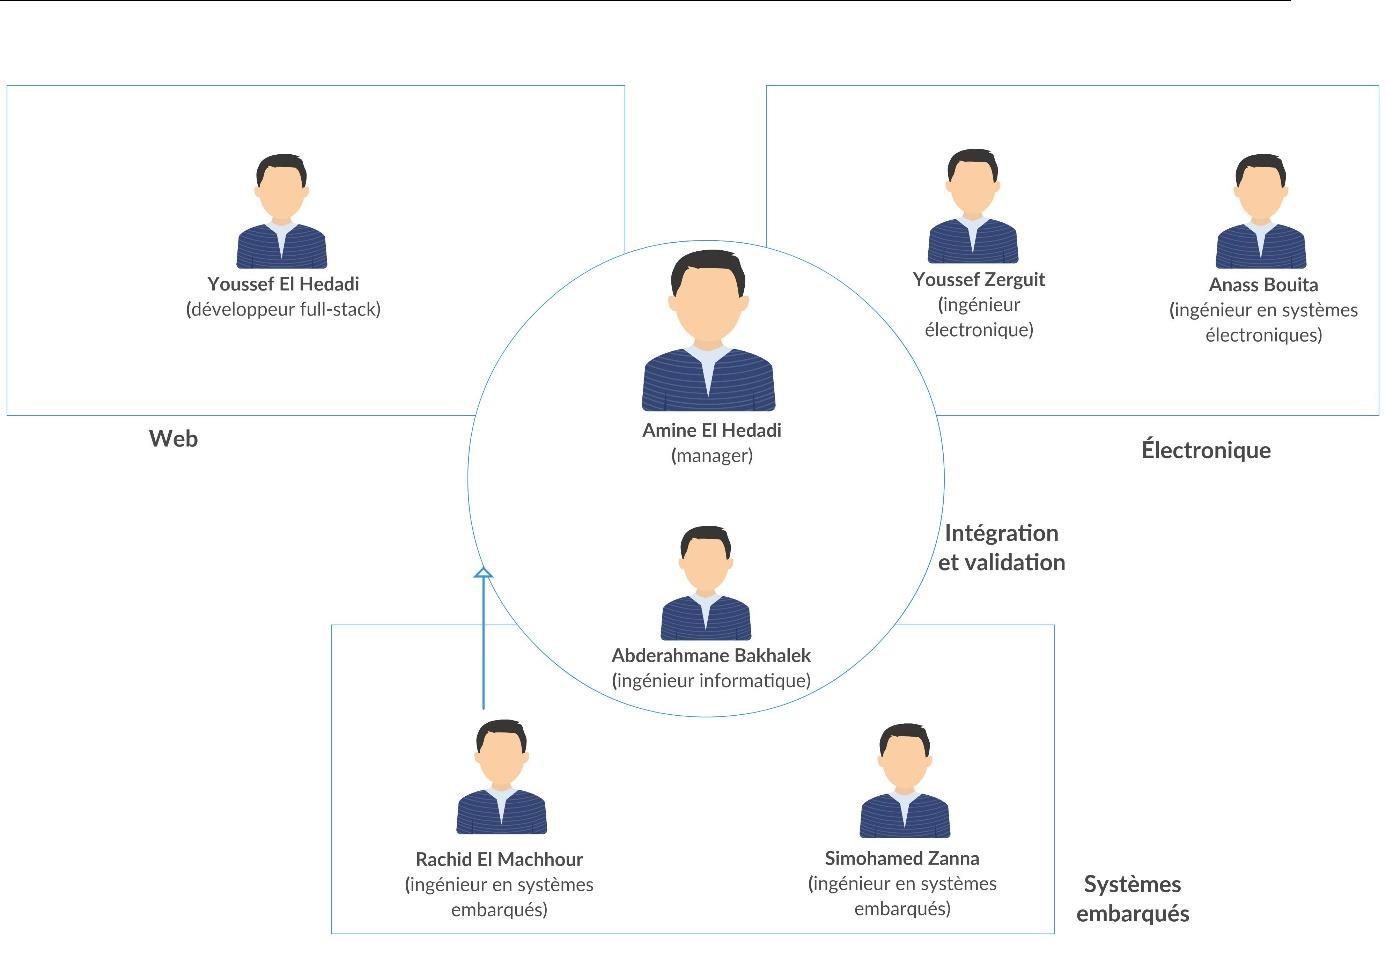
\includegraphics[width=12cm]{images/archi.png}
		\caption{Structure de l'équipe Esvitech}
		\label{fig:figure}
	\end{center}
\end{figure}

\subsection{Fonctionnement}
L'entreprise tourne au rythme de projets contractuels avec différents acteurs
économiques du Maroc. Chacun de ces projets est spécifique aux besoins de la société
cliente. La structuration en départements (web, électronique, logiciels embarqués,
...) permet à toute l'équipe de travailler en parallèle sur différents aspects du même
projet.

\section{L'entreprise dans son secteur d'activité}

\subsection{Le portefeuille d'Esvitech}
Il sera donné dans cette partie un court tour d'horizon des services fournis par
la société.
\subsubsection{La télémétrie}
Associant une technologie de capteurs et un logiciel intuitif (figure 1.2), le
système de surveillance continue aide les entreprises à répondre aux exigences réglementaires et à éviter les pertes ou altérations de produits.
Ce type de logiciels permet de réduire considérablement les coûts liés à la
surveillance "sur place" et automatise l'enregistrement des événements. Cela per-
met également d'intégrer un système d'alarme automatique ainsi qu'un monitoring
continu, qu'il serait très compliqué d'obtenir par la voie classique.


\begin{figure}[H]
	\begin{center}
		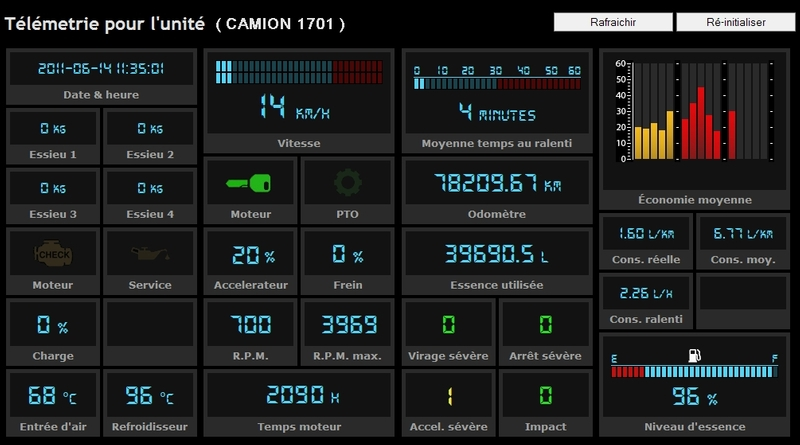
\includegraphics[width=12cm]{images/telem.png}
		\caption{Exemple d'une interface de télémétrie}
		\label{fig:figure}
	\end{center}
\end{figure}

\subsubsection{L'affchage dynamique}
Il s'agit de l'un des services phares d'Esvitech, du moins pendant la période
de mon stage. Esvitech propose à des companies de tout domaine d'activités une
solution d'affichage sur écran hautement conffigurable et personnalisable. Il est ainsi
possible de rentabiliser au maximum le support d'affichage en y disposant de multiples informations aux formats divers (documents, images, vidéos, fux RSS, cartes
géographiques, ...). Ayant effectué mon stage en surcouche de cette application, j'en
détaillerai le principe plus loin.

\subsubsection{Les ERP}
L'expertise d'Esvitech s'étend également au domaine des progiciels de gestion
intégrés (ou ERP pour Enterprise Resource Planning ). Un exemple est EAGRO-
ERP, un progiciel dédié à la gestion et le suivi d'exploitations agricoles. Il permet de
faire le suivi parcelle par parcelle de l'exploitation. Comme tout ERP, il permet une
traçabilité en temps réel de la production, mais également une gestion des stocks,
des achats et des ventes.

\section{Déroulement du stage}
Mon stage d'application s'est étalé sur deux mois, entre le 14 juillet et le 15
septembre 2017. Cette période a été consacrée au développement de trois appli-
cations, après une journée de prise de contact avec le personnel et les projets en
cours.
Les deux premières semaines (annexe A) ont servi à prendre en main Qt et
QML, mais également à développer une carte de télémétrie de groupes électrogènes.
Avec le projet d'analyse de conduite d'Esvitech comme arrière-plan, la suite du stage
a concerné le développement de deux applications de visualisation de signaux : l'une
sous la forme de graphes et l'autre sous forme animée et dynamique.
\section*{Conclusion}

La startup Esvitech est une société moderne qui offre son savoir-faire techno-
logique à de nombreuses sociétés marocaines, aux secteurs d'activité divers. Cette
pluridisciplinarité caractérise également le personnel de l'entreprise, en plus d'une
structure fexible et collaborative.

\chapter{Problématique et étude théorique des
	composants logiciels}
\section{Problematique}
\subsection{Introduction}
Nous commencerons ce chapitre par une définition de la Lecture Automatique de
Plaques d’Immatriculation (LAPI) et la technique de la reconnaissance de caractères. Après
ceci, nous allons présenter les applications LAPI. Nous finirons ce chapitre par exposer
quelques exemples de systèmes LAPI.
\subsection{Lecture automatique de plaques d’immatriculation}
La lecture automatique de plaques minéralogiques ou Lecture Automatisée de Plaques
d’Immatriculation (LAPI) est une méthode d'identification qui utilise des techniques de
traitement d'images et de vision par ordinateur pour extraire le numéro d’identification d’après
l’image de la plaque sous format de caractères en code ASCII
\begin{figure}[H]
	\begin{center}
		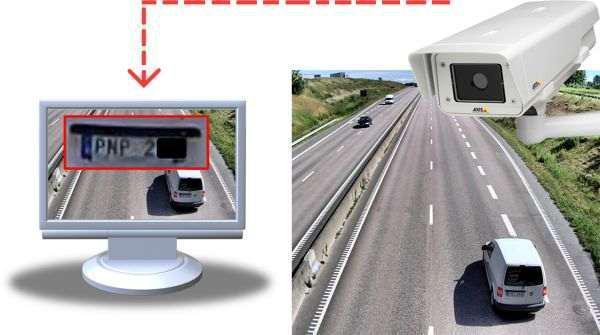
\includegraphics[width=12cm]{images/chaine.png}
		\caption{la chaine de transformation pour obtenir les caractères ASCII}
		\label{fig:figure}
	\end{center}
\end{figure}
Un système (LAPI) permet un dialogue avec un grand nombre de périphériques:

--Camera

--Radar de vitesse

--Lasers de detection

Comme nous nous intéressons aux plaques d’immatriculation marocaines,
nous commençons par donner quelques explications de base concernant les plaques
d’immatriculation de véhicules au Maroc :

\subsubsection{Caractéristiques des plaques Marocaines}
\begin{figure}[H]
	\begin{center}
		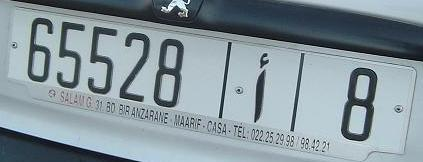
\includegraphics[width=12cm]{images/matricule.png}
		\caption{Matricule Marocain}
		\label{fig:figure}
	\end{center}
\end{figure}

L’immatriculation actuelle des véhicules enregistrés au Maroc respecte une nouvelle
norme d’immatriculation à compter de l’an 2000. Cette nouvelle configuration est
composée d’une série de cinq chiffres allant de 1 à 99 999 qui correspond au numéro
d’enregistrement de la voiture. Une lettre de l’alphabet arabe est incrémentée au
milieu de la plaque de contrôle, ce dernier prend en compte le numéro
d’enregistrement de l’automobile. Pour conclure la combinaison alphanumérique de la
plaque minéralogique marocaine, le nouveau système d’immatriculation en vigueur
actuellement dans le royaume chérifien termine la combinaison par l’identifiant de la
préfecture d’émission de la plaque. Ces numéros vont de 1 à 88
Basé sur les caractéristiques ci-dessus, nous proposons, dans la section
suivante, la technique utilisée dans ce système pour la reconnaissance optique de
caractères.

\subsubsection{La technique de la reconnaissance optique de caractères}
La lecture automatique de plaques minéralogiques utilise la
reconnaissance optique de caractères (OCR) sur des images prises par des caméras.
Certaines plaques d'immatriculation varient dans la taille des caractères et leur
position. Les systèmes de lecture automatique de plaques minéralogiques doivent
savoir traiter ces différences pour être vraiment efficaces. Les systèmes les plus
évolués savent gérer les variations entre pays, bien que beaucoup de programmes
soient spécifiques à un pays.

\subsection{Algorithmes du système LAPI}
Cinq étapes doivent être réalisées pour que le logiciel puisse identifier
une plaque d'immatriculation :

\begin{enumerate}
	\item Localisation de la plaque : responsable de trouver et d'isoler la plaque sur
	l'image.
	\item Orientation et dimensionnement de la plaque : compensation de
	l'orientation de travers de la plaque et ajustement des dimensions à la taille
	nécessaire.
	\item Normalisation : ajustement de l'intensité et du contraste de l'image.
	\item Segmentation des caractères : localisation des caractères sur la plaque.
	\item Reconnaissance optique de caractères.
	
\end{enumerate}

La complexité de chacune des étapes du programme détermine la précision du
système. Pendant la troisième phase (normalisation), certains systèmes utilisent des
techniques de détection de contour pour augmenter le contraste entre les lettres et lacouleur de fond de la plaque. Un filtre numérique peut aussi être utilisé pour réduire
le bruit » visuel de l'image.
\subsection{Difficultés des systèmes LAPI}
Le logiciel doit être capable de gérer un grand nombre de difficultés
possibles.
Parmi ces difficultés :
\begin{itemize}
	\item Une mauvaise résolution de l'image, souvent parce que la plaque est trop
	loin, mais parfois à cause de l'utilisation d'une caméra de mauvaise qualité.
	\item Des images floues, souvent à cause du mouvement, très fréquentes sur les
	installations mobiles.
	\item Un mauvais éclairage et un faible contraste à cause d'une surexposition,
	d'un reflet, ou d'ombres.
	\item Un objet obscurcissant une partie de la plaque, souvent une barre de
	remorquage, ou de la poussière sur la plaque.
	\item Une police de caractère trop originale, chose fréquente sur les plaques
	fantaisie (certains pays interdisent de telles plaques, ce qui élimine le
	problème).
\end{itemize}

\subsection{Applications des systèmes LAPI}
La lecture automatique de plaques minéralogiques peut également être
utilisée pour :
\begin{itemize}
	\item Les passages de frontière.
	\item Les stations-services (enregistrement quand un client part sans payer).
	\item Le contrôle d'accès des parkings ou routes privées: ouverture automatique, ou
	enregistrement de l'entrée.
	\item Un outil de marketing pour enregistrer les modes de consommation.
	\item Les systèmes de gestion de la circulation, qui calculent la vitesse de
	circulation en mesurant le temps entre les passages devant deux points de
	lecture.
	\item Comparer les plaques d'immatriculations au Fichier des véhicules volés.
	\item Pour certaines applications, le système peut être associé à d'autres algorithmes
	de
	reconnaissance de type facial ou de véhicule.
\end{itemize}
\subsection{Les différents systèmes existants}
De nos jours, il existe de nombreux systèmes de la reconnaissance de plaques
d’immatriculation, tels que :
\subsubsection{AutoVu}
Est le système de reconnaissance de plaques d’immatriculation (RAPI) sur IP
de Security Center, la plate-forme de sécurité unifiée de Genetec\\
ses avantages :
\begin{itemize}
\item Obtenez des lectures de plaques d’immatriculation précises.
\item Assurez des performances interrompues.
\item
Fournisseur de solutions de RAPI complètes.
\item
Unification avec la vidéosurveillance.
\item
Combinez la RAPI fixe.
\end{itemize}
\subsubsection{LAPI ENGINE}
Le produit LAPI ENGINE représente le cœur technologique permettant la
Lecture Automatique de Plaques d’Immatriculation (LAPI - ANPR). Principalement
dédiée à la traçabilité de véhicules, LAPI ENGINE est un produit autonome pouvant
s’adapter à un large éventail d’applications.\\
ses avantages
\begin{itemize}
\item Possibilité de crypter les données (images et n plaques) avec un système de
gestion de clé unique.
\item Lecture de tous types de plaques réfléchissantes aux infrarouges ou non.
\item Maintenance et intervention sur tout le territoire Français (Télé-maintenance
possible).
\item  Moteur LAPI fonctionnant sur Windows, Linux.
\end{itemize}

\subsubsection{SeeTec}
Est un module d'extension de SeeTec Cayuga qui permet la reconnaissance
automatique de plaques d'immatriculation de véhicules à l'arrêt ou en mouvement.\\
ses avantages :
\begin{itemize}
\item Il peut lire des formats de plaques internationaux, même en caractères arabes
et cyrilliques, jusqu'à huit voies de circulation par serveur.
\item la reconnaissance des plaques d'immatriculation s'effectue en continu ou est
pilotée par un déclencheur.
\item SeeTec peut être utilisé avec chaque caméra IP prise en charge par SeeTec et
intégrée au système. Même dans des conditions de luminosité difficiles.
\end{itemize}

\subsubsection{Asia Vision Technology Limited (AVT)}
Est le premier fournisseur mondial de solutions technologiques et de solutions
de gestion intelligente des véhicules et des conteneurs. AVT a été un pionnier dans le
développement et la fourniture de la technologie de reconnaissance optique de
caractères (OCR).\\
Avantages d’Asia Vision
\begin{itemize}
\item Le système détecte, reconnaît et vérifie automatiquement la plaque
d'immatriculation, à la fois alphanumérique et non alphanumérique des
véhicules.
\item Le système a réussi à reconnaître les plaques d'immatriculation de 20 pays dans
plusieurs langues, y compris l'anglais, le chinois, le coréen, le japonais, le
thaïlandais, l'espagnol et le portugais.
\end{itemize}
\subsubsection{AGL (Application de Gestion LAPI)}
Est basée essentiellement sur la technologie LAPI, le but d’AGL est de
permettre l’automatisation de processus pour les forces de l’ordre, notamment par
l’acquisition de données au travers de capteurs dédiés. Ces données peuvent ensuite
être interprétées de différentes façons, allant de la notification simple d’information
(en croisant avec des données internes), à une aide à la verbalisation électronique
\begin{itemize}
\item Elle permet de rassembler, traiter, et extraire les données. Elle est composé de
l’ensemble des capteurs (optiques, RFID, laser, GPS) qui collectent des données de
voirie de manière automatique, semi-automatique ou manuelle.
\item Elle permet d’acquérir des données, et de les utiliser sur le terrain. Elle est relié
d’une part aux services nationaux, aux prestataires tiers, aux services locaux des
collectivités et d’autre part aux systèmes AGL Capture.
\end{itemize}

\subsubsection{Système LAPI-Pryncar}
Est enregistrée les plaques d’immatriculation dans son champ de vision.
L’immatriculation du véhicule peut ainsi être lue et comparée au fichier des véhicules
enregistrés dans le cadre d’un contrôle d’accès ou d’une recherche de véhicule.
\begin{itemize}
\item Contrôle d’accès : Parkings privés ou publics, surveillance de sites,
péages, stations-service, etc.
\item Gestion de trafic, sécurité routière : Villes embouteillées, régulation du
trafic, etc.
\item Capteur LAPI Fixe autonome.
\item Appli Pryncar pour Smartphone.
\end{itemize}


\paragraph{Nous avons trouvée beaucoup systèmes, nous avons citée quelques-un d’entre
	elles et ses différents systèmes proposés sont basés sur des propriétés différentes. Des
	techniques utilisent des règles simples basées sur des méthodes existantes pour la
	détection et la reconnaissance des plaques d’immatriculation.}

\section{étude théorique des composants logiciels}
\subsection*{le portage du linux :en utilisant le buildroot}

Les ordinateurs embarqués fonctionnant sous le système d’exploitation Linux sont
massivement présents dans les technologies modernes (transports, multimédia, téléphonie
mobile, appareils photos ...). Contrairement aux versions de Linux destinées aux ordinateurs
personnels et aux serveurs, les différents systèmes Linux embarqués sont conçus pour des
systèmes aux ressources limitées. Les systèmes embarqués sous Linux disposent
généralement de peu de RAM et utilisent fréquemment de la mémoire flash plutôt qu'un
disque dur. Comme ils sont souvent dédiés à un nombre de tâches réduites sur une cible
matérielle bien définie, ils utilisent plutôt des versions du noyau Linux optimisées pour des
contextes précis
\subsection{Introduction}
Dans le domaine de l'embarqué, on se retrouve souvent en situation de devoir reconstruire un
système complet à partir des sources, pour une architecture cible souvent différente de celle
de l’hôte. La crosscompilation et l'organisation d'un système embarqué sont des étapes
longues et fastidieuses, surtout lorsque les éléments du système à compiler nécessitent des
adaptations. Il existe heureusement des outils libres qui simplifient et accélèrent cette tâche,
en proposant généralement des fonctionnalités complémentaires intéressantes. Buildroot est
un de ces outils qui simplifie et automatise le processus de construction d'un système Linux
complet pour un système embarqué. Afin d'atteindre cet objectif, Buildroot est capable degénérer une chaîne de compilation croisée, un système de fichiers (rootfs), une image du
noyau Linux (kernel) et un chargeur de démarrage (firmware/bootloader) pour la cible. Il
prend en charge de nombreux processeurs et leurs variantes (x86, PowerPC, MIPS, ARM,
NIOS, etc). Il est également livré avec des configurations par défaut pour un grand nombre de
cartes disponibles sur le marché.
\subsection{la configuration}

Buildroot est techniquement un ensemble de Makefiles
définissant, en fonction des options paramétrées par l'utilisateur, la manière de compiler
chaque paquet sélectionné avec des options particulières. Il construit finalement une
distribution complète et cohérente dont chaque composant a été compilé. Il possède un outil
confortable de configuration, basé et très similaire à celui du noyau Linux : menuconfig, que
l'on retrouve également avec Busybox, uClibc et qui peut être utilisé dans tout projet.

où il y a deux types du fichier RaspberryPi defconfig dans le  Buildroot :\\
pour les modeles A, B, A+ or B+:
 make raspberrypi defconfig
 
pour le modele ZERO (model A+ in smaller form factor):
 make raspberrypi0 defconfig
 
pour le modele  2 B:
 make raspberrypi2 defconfig
 
pour le modele 3 B and B+:
 make raspberrypi3 defconfig
 
 
\subsubsection{La commande Make}

La commande make effectue généralement les étapes suivantes : téléchargement des fichiers
sources (si nécessaire); configuration, compilation et installation de la chaîne de compilation
croisée configuration, compilation, corrections (application des patchs) et installation des
paquets cibles sélectionnées; construction d’une image du noyau construction d’une image
de bootloader; création d’un système de fichiers racine (rootfs) dans les formats sélectionnés.
\subsection{l'ajout de l'image à la carte mémoire..}

~/buildroot\$ sudo dd if=output/images/rpi3-sdcard.img of=/dev/sdb bs=1M
\section{Conclusion}
Nous avons vu dans ce chapitre la notion de Lecture Automatique de Plaques
Minéralogique et ses différents algorithmes qui doivent être réalisés pour que le
logiciel puisse identifier une plaque d'immatriculation et les difficultés qui en résultent.
Comme nous le verrons quelques exemples de système existants.


\chapter{Traitement D'images}
\section{Introduction}
Le traitement d’images est un domaine très vaste qui a connu, et qui connaît encore,
un développement important depuis quelques dizaines d’années.

Nous ayons désignée par traitement d'images numériques l'ensemble des techniques
permettant de modifier une image numérique afin d'améliorer ou d'en extraire des
informations.

Dans ce chapitre, nous abordons les notions de base nécessaires à la compréhension
des techniques de traitement d’images. Ensuite, nous allons donner un aperçu sur les
différentes techniques connues dans ce domaine.


\section{Définition du traitement d’images}
Le traitement d'images est une discipline de l'informatique et des mathématiques
appliquées qui étudie les images numériques et leurs transformations, dans le but
d'améliorer leur qualité ou d'en extraire de l'information. [9]
La compréhension du traitement d'images commence par la compréhension de ce
qu'est une image. Le mode et les conditions d'acquisition et de numérisation des images
traitées conditionnent largement les opérations qu'il faudra réaliser pour extraire de
l'information. En effet, de nombreux paramètres entrent en compte, les principaux étant :

\begin{itemize}
\item La résolution d'acquisition et le mode de codage utilisé lors de la numérisation, qui
déterminent le degré de précision des éventuelles mesures de dimensions.
\item Les réglages optiques utilisés, (dont la mise au point) qui déterminent par exemple la
netteté de l'image.
\item Les conditions d'éclairage, qui déterminent une partie de la variabilité des images
traitées.
\end{itemize}
Quelques exemple de types d'informations qu'il est possible d'obtenir d'une image
numérique :
\begin{itemize}
\item La luminance moyenne.
\item  Le contraste moyen.
\item La couleur prédominante.
\item  Le taux d'acuité moyen (précis ou flou).
\item  Le taux d'uniformité des couleurs.
\item  La présence ou l'absence de certains objets.

\end{itemize}

\section{l'Image}
Une image est avant tout un signal 2D (x, y), qui représente souvent une réalité 3D
(x, y, z). D'un point de vue mathématique, une image est une matrice de nombres
représentant un signal, plusieurs outils permettent de manipuler ce signal. [10]
Il existe trois principaux types d'images :
\begin{enumerate}
\item  Les images binaires (uniquement en noir et blanc) et dont la valeur soit 0 soit 1.
\item  Les images en niveaux de gris, dont la valeur appartient à l’ensemble ,0,1,...,255-.
\item Les images couleurs.

\end{enumerate}


\section{Représentation d’image}
Les images numériques, destinées à être visualisées sur les écrans d'ordinateur, se
divisent en 2 grandes classes :

\begin{itemize}
\item Les images matricielles
\item  Les images vectorielles.
\end{itemize}

\subsection{Image matricielle}
Encore appelée image bitmap, Une image matricielle est formée d’un assemblage de
points ou de pixels.

Nous parlons sur de points lorsque ces images sont imprimées ou destinées à
l’impression (photographies, publicités, cartes etc.) et nous parlons sur de pixels pour les
images stockées sous forme « binaire » ou numérique.
\subsection{Les images vectorielles}

Une image vectorielle en informatique, est une image numérique composée d’objets
géométriques individuels (segments de droite, polygones, arcs de cercle, etc.) définis chacun
par divers attributs de forme, de position, de couleur, etc. (définis de manière
mathématique).

Par exemple, une image vectorielle d’un cercle est définie par des attributs de types :
position du centre, rayon, etc....

\section{Acquisition d'une image}

L’acquisition d’images constitue un des maillons essentiels de toute chaîne de
conception et de production d’images. Pour pouvoir manipuler une image sur un système
informatique, il est avant tout nécessaire de lui faire subir une transformation qui la rendra
lisible et manipulable par ce système. Le passage de cet objet externe (l’image d’origine) à sa
représentation interne (dans l’unité de traitement) se fait grâce à une procédure de
numérisation. Ces systèmes de saisie, dénommés optiques, peuvent être classés en deux
catégories principales:

\begin{itemize}
\item  Les caméras numériques.
\item  Les scanners.
\end{itemize}
\section{Caractéristiques d’une image numérique}

L’image est un ensemble structuré d’informations caractérisé par les paramètres
suivants :
\subsection{Dimension}
C’est la taille de l’image. Cette dernière se présente sous forme de matrice dont les
éléments sont des valeurs numériques représentatives des intensités lumineuses (pixels). Le
nombre de lignes de cette matrice multiplié par le nombre de colonnes nous donne le
nombre total de pixels dans une image.
\subsection{Résolution}

C’est la clarté ou la finesse de détails atteinte par un moniteur ou une imprimante
dans la production d’images. Sur les moniteurs d’ordinateurs, la résolution est exprimée en
nombre de pixels par unité de mesure (pouce ou centimètre). Nous utilisons aussi le mot
résolution pour désigner le nombre total de pixels affichables horizontalement ou
verticalement sur un moniteur; plus grand est ce nombre, meilleure est la résolution
\subsection{bruit}
Un bruit (parasite) dans une image est considéré comme un phénomène de brusque
variation de l’intensité d’un pixel par rapport à ses voisins, il provient de l’éclairage des
dispositifs optiques et électroniques du capteur.

\subsection{Histogramme}
L’histogramme des niveaux de gris ou des couleurs d’une image est une fonction qui
donne la fréquence d’apparition de chaque niveau de gris (couleur) dans l’image. Il permet
de donner un grand nombre d’information sur la distribution des niveaux de gris (couleur) et
de voir entre quelles bornes est repartie la majorité des niveaux de gris (couleur) dans le cas
d’une image trop claire ou d’une image trop foncée.

Il peut être utilisé pour améliorer la qualité d’une image (Rehaussement d’image) en
introduisant quelques modifications, pour pouvoir extraire les informations utiles de celle-ci.

Pour diminuer l’erreur de quantification, pour comparer deux images obtenues sous
des éclairages différents, ou encore pour mesurer certaines propriétés sur une image, on
modifie souvent l’histogramme correspondant.

\subsection{Luminance}
C’est le degré de luminosité des points de l’image. Elle est définie aussi comme étant
le quotient de l’intensité lumineuse d’une surface par l’aire apparente de cette surface, pour
un observateur lointain, le mot luminance est substitué au mot brillance, qui correspond à
l’éclat d’un objet. Une bonne luminance se caractérise par :
\begin{itemize}
\item Des images lumineuses (brillantes).
\item Un bon contraste: il faut éviter les images où la gamme de contraste tend vers le
blanc ou le noir, ces images entraînent des pertes de détails dans les zones sombres
ou lumineuses.
\item L’absence de parasites.

\end{itemize}
\subsection{Contraste}
C’est l’opposition marquée entre deux régions d’une image, plus précisément entre
les régions sombres et les régions claires de cette image. Le contraste est défini en fonction
des luminances de deux zones d’images
\subsection{Images à niveau de gris}
Le niveau de gris est la valeur de l’intensité lumineuse en un point. La couleur du
pixel peut prendre des valeurs allant du noir au blanc en passant par un nombre fini de
niveaux intermédiaires. Donc pour représenter les images à niveaux de gris, nous pouvons
attribuer à chaque pixel de l’image une valeur correspondant à la quantité de lumière
renvoyée. Cette valeur peut être comprise par exemple entre 0 et 255. Chaque pixel n’est
donc plus représenté par un bit, mais par un octet. Pour cela, il faut que le matériel utilisé
pour afficher l’image soit capable de produire les différents niveaux de gris correspondant.
Le nombre de niveaux de gris dépend du nombre de bits utilisés pour décrire la
"couleur" de chaque pixel de l’image. Plus ce nombre est important, plus les niveaux
possibles sont nombreux.
\subsection{Images en couleurs}
Même s’il est parfois utile de pouvoir représenter des images en noir et blanc, les
applications multimédias utilisent le plus souvent des images en couleurs. La représentation
des couleurs s’effectue de la même manière que les images monochromes avec cependant
quelques particularités. En effet, il faut tout d’abord choisir un modèle de représentation.
Nous pouvons représenter les couleurs à l’aide de leurs composantes primaires. Les
systèmes émettant de la lumière (écrans d’ordinateurs,...) sont basés sur le principe de la synthèse additive: les couleurs sont composées d’un mélange de rouge, vert et bleu (modèle
R.V.B).
\section{Principales étapes de traitement d’images}
Il n'existe pas de méthode de traitement d'images générale à tous les domaines
d'application possibles. Il faut en général employer des algorithmes spécifiques. Ces derniers
sont souvent des combinaisons de techniques classiques (segmentation, classification,
reconnaissance de frontières, etc.). De manière schématique, toute méthode de traitement
d'images comprend 3 étapes majeures :
\begin{itemize}
\item  Prétraitement des images.

\item  Amélioration des images.

\item Analyse des images.
\end{itemize}

\subsection{Prétraitements}

Ils préparent l'image pour son analyse ultérieure. Il s'agit souvent d'obtenir l'image
théorique que l'on aurait dû acquérir en l'absence de toute dégradation. Ainsi, ils peuvent
par exemple corriger :
\begin{itemize}
\item Les défauts radiométriques du capteur : non linéarité des détecteurs, diffraction de
l'optique, etc.
\item
Les défauts géométriques de l'image dus au mode d'échantillonnage spatial, à
l'oblicité de la direction de visée, au déplacement de la cible, etc.
\item
Le filtrage ou réduction de fréquences parasites, par exemple dus à des vibrations du
capteur.
\item Les dégradations de l'image dues à la présence de matière entre le capteur et le
milieu observé.
\end{itemize}
\subsection{Amelioration D'image}
Elle a pour but d'améliorer la visualisation des images. Pour cela, elle élimine / réduit
le bruit de l’image et/ou met en évidence certains éléments (frontières, etc.) de l'image. Elle
est souvent appliquée sans connaissance à priori des éléments de l'image. Les principales
techniques sont :
\begin{itemize}
\item L'amélioration de contraste.
\item Le filtrage linéaire (lissage, mise en évidence des frontières avec l'opérateur "Image -
Image lissée", etc.) et transformée de Fourier pour faire apparaître / disparaître
certaines fréquences dans l'image.
\item
Filtrage non linéaire (filtres médians, etc.) pour éliminer le bruit sans trop affecter les
frontières, etc.

\end{itemize}

\subsection{Analyse d'image}
Le but de l’analyse d’images est d'extraire et de mesurer certaines caractéristiques
de l'image traitée en vue de son interprétation. Ces caractéristiques peuvent être des
données statistiques sur des comptes numériques (moyenne, histogramme, etc.), ou sur des
données dérivées (ex. dimensions, ou orientation d’objets présents dans l’image). En
général, le type d'information recherché dépend du niveau de connaissance requis pour
interpréter l'image. Les applications dans le domaine du guidage et de la télédétection
nécessitent souvent des connaissances différentes et de plus haut niveau (ex., cartes 3-D)
que dans les domaines du médical, de la géologie, du contrôle de qualité, etc. Ainsi, un robot
en déplacement ne nécessite pas le même type d'information qu'un système utilisé pour
détecter la présence de matériaux défectueux. Pour ce dernier, il faut prendre uniquement
la décision "non défectueux ou défectueux". Cette décision peut être prise à partir d'un
"raisonnement" plus ou moins complexe (e.g. détection de la présence de raies d'absorption
caractéristiques d'une impureté). Pour le robot, il faut simuler le processus décisionnel d’un
individu en déplacement, ce qui nécessite au préalable de reconstituer une carte du lieu de
déplacement en temps réel, avec les obstacles à éviter.
\section{Types de données manipulée}
Le
traiteur
d'image
dispose
principalement
d'images
numériques,
donc
échantillonnées. Il dispose également de données intermédiaires de diverses natures : cartes
de régions, listes de points connexes, tableaux de valeurs mesurées, etc.

En ce qui concerne les images proprement dites, la représentation la plus utilisée est
celle d'un tableau à 2 dimensions composé d'un ensemble de lignes et de colonnes.

Chaque cellule du tableau, appelée pixel, contient une valeur quantifiée. Cette valeur
est une sémantique dépendant du type de signal qu'elle code (intensité lumineuse du point,
distance à un point de référence, ou numéro de la région d'appartenance par exemple).

Dans le cas des images 3D d'IRM, la représentation n'est plus un tableau à 2 dimensions mais
un tableau à 3 dimensions.
\section{Opérateurs de traitement d’image}
Par analogie avec les opérateurs mathématiques, on appelle opérateurs de
traitement d'images des traitements plus ou moins complexes prenant en entrée une image
ou un ensemble d'informations relatif à une image, et produisant une image ou un ensemble
d'informations relatif aux données initiales.

Nous avons classé généralement les opérateurs en différentes familles, en fonction
des informations qu'ils acceptent en entrée et qu'ils fournissent en sortie, et en fonction des
transformations qu'ils font subir aux données. Ainsi, par exemple, on distingue (cette liste
est loin d'être exhaustive) :

\subsection*{Opérateurs image - image} 
\begin{itemize}
\item  Opérateurs de modifications pixel à pixel (aussi appelés opérateurs point à point) :
changement de la dynamique de l'image, opérateurs binaires pixel à pixel (et, ou, or,
etc.).
\item 
Opérateurs locaux (traitent les pixels en fonction de leur voisinage) : opérateurs de
flou, opérateurs morphologiques (érosion, dilatation, squelette), opérateurs de
détection de contours.
\item 
Opérateurs dans l'espace fréquentiel : opérateurs de réduction du bruit, filtres
passe-bande (souvent utilisés en première approche pour améliorer l'image, on les
appelle alors des opérateurs de prétraitement).
\item  Opérateurs globaux : calcul des distances.
\item Opérateurs de croissance de régions : Ligne de partage des eaux.

\end{itemize}
\subsection*{Opérateurs image -ensemble d'informations}
\begin{itemize}
\item Opérateurs de segmentation en frontières, en régions.
\item  Opérateurs de classification de pixels.
\item  Opérateurs de calcul de paramètres.
\end{itemize}
\subsection*{Opérateurs ensemble d'informations -image}
\begin{itemize}
	\item 
	constructeurs d'image à partir d'une carte de régions ou d'une liste de frontières.
\end{itemize}
\paragraph{
Les parties suivantes s'attachent à détailler les différents opérateurs et leurs
applications habituelles, puis à présenter la manière dont ils sont combinés pour construire
une application de traitement d'images.}

\subsection{Opérateurs locaux}
Il faut alors utiliser des opérateurs de traitement plus complexes scindés bien
souvent en deux sous-catégories :

- Les filtres linéaires.

- Les filtres non linéaires.


La première sous-catégorie comprend tous les opérateurs pouvant exprimer leur
résultat comme une combinaison linéaire des niveaux de gris d'un voisinage de l'image. Ces
filtres possèdent des caractéristiques spectrales, on parle ainsi de filtre passe-bas (l'image
devient floue) ou de filtre passe-haut (les contours ressortent).

La deuxième sous-catégorie comprend le domaine de la morphologie mathématique,
ainsi que d'autres traitements comme les détecteurs de points caractéristiques, l'opérateur
de Di-Zenzo (détecteur de contour généralisé au cas couleur), le filtre Retinex, ainsi que les
opérateurs homomorphiques (ceux qui travaillent sur le logarithme de l'image).

Nous avons l'habitude de voir un détecteur de contours s'appliquer après un filtre
linéaire passe-bas... qui rend l'image floue ! La plupart du temps il faut combiner
astucieusement filtre non linéaire et filtre linéaire afin de détecter ce que l'on souhaite tout
en faisant abstraction du bruit.

Une fois le bruit éliminé et l'image restaurée afin de compenser les déformations
introduites par le milieu de transmission et l'optique d'acquisition, nous pouvons passer à
l'étape de segmentation qui doit permettre de réaliser une partition de l'image en
ensembles connexes homogènes.

Il existe deux grandes catégories de segmentations :

\begin{itemize}
\item La segmentation de région.
\item  La segmentation de contour : nous nous trouvons alors  confronté à un problème de
représentation du résultat par des primitives simples.
\end{itemize}
La segmentation orientée contour connaît de nombreux progrès autour de
l'utilisation de contours actifs ou des ensembles de niveaux. L'introduction d'aspects
probabilistes (chaîne de Markov et champs de Markov) a permis de travailler en réduisant la
connaissance a priori nécessaire pour obtenir un traitement satisfaisant.


Dans cette étape nous retrouvons souvent une partie de classification des pixels en
classes. Nous essayons de regrouper au sein d'un même ensemble, aussi appelé classe, les
pixels présentant une même caractéristique : niveau de gris compris dans un certain
intervalle ou dérivée seconde supérieure à un certain seuil.
\subsection{Filtres linéaires}
Un filtre linéaire transforme un ensemble de données d'entrée en un ensemble de
données de sortie selon une opération mathématique appelée convolution. Lorsqu'il s'agit
de données numérisées comme dans le cas du traitement d'image, la relation entre les
valeurs des pixels de sortie et celle des pixels d'entrée est décrite par un tableau de
nombres, généralement carré, appelé matrice de convolution. Le temps de calcul est
souvent réduit lorsqu'on veut séparer un filtre en deux filtres dont la convolution mutuelle
permet de le reconstituer. Cette remarque est utilisée en particulier pour créer un filtre à
deux dimensions à partir de deux filtres à une seule dimension (vecteurs) dans le sens
horizontal et le sens vertical.

\subsubsection{Lissage}
Ceux-ci sont des filtres passe-bas qui coupent plus ou moins les plus hautes
fréquences. Ils sont utilisés pour atténuer les bruits d'origines les plus diverses qui polluent
l'information, en particulier dans la détection de contours considérée ci-après.
Techniquement, il s'agit de traductions discrètes de filtres continus qui, comme ceux-
ci, ne modifient pas le niveau global du signal. Les termes de la matrice de convolution sont
donc généralement des entiers à diviser par leur somme.

\begin{itemize}
\item Filtre uniforme : il est obtenu par convolution de deux filtres unidimensionnels
rectangulaires. Toutes les composantes de la matrice ont la même valeur.
L'imperfection de ce filtre réside dans le fait qu'il introduit des déphasages.
\item
Filtre pyramidal : la convolution d'un filtre rectangulaire avec lui-même conduit à un
filtre triangulaire grâce auquel les phases ne sont plus modifiées. Le filtre pyramidal
est obtenu à partir de filtres triangulaires dans les deux directions.
\item
Filtre gaussien: ce filtre très populaire utilise la loi de probabilité de Gauss (voir Loi
normale multidimensionnelle). Des approximations de plus en plus précises peuvent
être obtenues, selon le théorème central limite par itération de l'un des filtres
précédents.
\end{itemize}
\subsubsection{Détection de contours}
Ces filtres transforment l'image d'entrée en une image noire sauf aux points où un
contour est détecté qui est marqué en blanc. Les valeurs absolues importent peu, il est sans
intérêt de changer d'échelle comme pour un lissage.

La détection est basée sur la dérivation selon les deux coordonnées. Si on considère
classiquement les signaux comme des sommes de sinusoïdes, la dérivation apparaît comme
un filtre passe-haut qui introduit donc du bruit à l'origine de faux contours. Pour l'amateur il
est recommandé, avant d'utiliser un filtre simple, d'atténuer ce bruit par passage dans un
filtre flou. Des méthodes plus élaborées ont été systématisées pour les professionnels.



\begin{itemize}
		\item 
	Filtre dérivées premières : Le filtre le plus simple consiste à calculer les différences
	entre pixels voisins sur les horizontales puis sur les verticales. Chaque extremum
	correspond à un point d'un contour.
		\item 
	Filtre de Prewitt : le filtre de Prewitt introduit un flou, chacune des deux matrices
	étant le produit du filtre dérivation dans la direction considérée par un filtre de flou
	rectangulaire selon l'autre direction.
		\item 
	Filtre de Sobel : la technique précédente est améliorée en remplaçant le filtre
	rectangulaire par un filtre triangulaire.
	\item 
	Filtre de Canny : c'est un filtre de Sobel précédé par un lissage gaussien et suivi par
	un seuillage. Ce filtre est conçu pour être optimal, au sens de trois critères.
		\item Filtre de Deriche : variante du filtre de Canny tout aussi efficace.
		\item  Filtre dérivées secondes : celles-ci se calculent simplement en différences finies et
	c'est maintenant un changement de signe qui correspond à un point d'un contour.
	On les utilise généralement à travers leur somme qui est le laplacien.
	\item 
	Filtre de Marr-Hildreth : le calcul du laplacien est précédé par un lissage gaussien
	avec deux variances ajustables pour filtrer les hautes fréquences.
	
\end{itemize}

\subsection{Opérateurs morphologiques}
La morphologie mathématique offre des opérateurs non linéaires particulièrement
utiles pour filtrer, segmenter et quantifier des images. Initialement destinée au traitement
des images binaires, elle a très vite été généralisée aux images à niveaux de gris, puis aux
images en couleurs et multi-spectrales.
La nature des opérateurs morphologiques fait qu'ils se prêtent bien au
développement de circuits électroniques spécialisés (ou bien à l'utilisation de FPGA) dans les
opérateurs morphologiques.
\subsection{Construction d’une application de traitement d’images}
Les objectifs des applications peuvent être de différentes natures :

-Détecter la présence d'un objet ou son absence.

-Calculer les caractéristiques d'un ou de plusieurs éléments de l'image.

Dans tous les cas, l'idée est, en partant d'une image initiale, d'en extraire des
informations. Pour cela, nous allons utiliser les opérateurs à la manière de « briques
logicielles », en les combinant et en les enchaînant. Ces techniques sont la base des
systèmes de vision industrielle.
De nombreuses briques sont disponibles permettant de créer des applications
complexes et évoluées.
\section{Reconnaissance d'objets}
La reconnaissance d'objets est une branche de la vision artificielle et un des piliers
de la vision industrielle. Elle consiste à identifier des formes pré-décrites dans une image
numérique, et par extension dans un flux vidéo numérique.

Il ne faut pas confondre reconnaissance d'objets (en anglais : « object recognition »
ou « shape recognition ») et reconnaissance de formes (« pattern recognition » en anglais).
La première s'attache à reconnaître des formes géométriques dans une image, alors que la
seconde cherche à identifier des motifs dans des données statistiques. La confusion vient du
fait qu'on utilise souvent la reconnaissance de formes comme technique appliquée à la
reconnaissance d'objets.

Tout d'abord objet d'algorithmes dirigés par l'homme, jusqu'en 1995 (tentatives de
reproduire par un algorithme un raisonnement humain d'identification, comme dans « un
vélo possède deux roues, un cadre... »), la reconnaissance d'objets a fait l'objet de progrès
importants par la suite au travers de la mise en œuvre de techniques d'apprentissage,
comme les séparateurs à vaste marge. Ces techniques visent à faire exploiter des bases
d'exemples positifs et négatifs (contre-exemples) par un algorithme de recherche de critères
discriminants, c'est-à-dire de critères permettant de séparer au mieux les exemples des
contre-exemples.
\section{Quelque exemples concrets de traitement d’image}
\begin{itemize}
\item Contrôle de présence/absence sur des chaînes de production, nous avons vérifié
en bout de chaîne avec une caméra vidéo la présence d'une pièce dans un ensemble
plus complexe. Pour cela bien souvent il suffit de faire un simple seuillage dans une
région spécifique.
\item
Contrôle du niveau de maturation des fruits sur une chaîne de
conditionnement . Il s'agit de reconnaître à la couleur et à la texture du fruit son
degré de maturité et donc la catégorie sous laquelle il sera emballé puis vendu.
\item
Construction et correction de cartes géographiques d'après des images
satellites ou des images aériennes . On recale d'après des informations
topographiques les images reçues, puis on les met sur la carte en correspondance
avec les informations trouvées dans l'image : voies de communication, voies et plans
d'eau, parcelles agricoles...
\item Surveillance et évaluation de la production agricole. Il est possible de
déterminer le degré de maturation des cultures, la quantité d'eau nécessaire pour
l'irrigation, le rendement moyen... Nous pouvons ainsi établir des prévisions à large
échelle de la récolte à venir.
\item
Reconnaissance de l'écriture . La reconnaissance de l'écriture manuscrite
progresse de jour en jour. Elle est suffisamment opérationnelle pour que la majorité
des adresses, même manuscrites, soient reconnues automatiquement sur le courrier
postal.
\item
Recherche d'image par le contenu . L'objectif de cette technique est de
rechercher, parmi une base de données d'images, les images similaires à une image
exemple, ou ayant certaines caractéristiques, par exemple rechercher toutes les
images comportant un vélo.
\item
Analyse de la vidéo. L'objectif de cette technique devenue une discipline depuis les
années 2000 (lorsque la puissance des processeurs peu onéreux et en particulier des
PC a permis des traitements puissants en temps réel) est d'interpréter les faits
observés à l'image afin de signaler ou d'enregistrer des faits marquants. Le plus
souvent, la caméra est fixe et observe les mouvements d'une scène. Les applications
sont nombreuses : protection des biens (détection d'intrusion, détection d'objet
abandonné ou déposé...), identification (biométrie faciale), Sécurité des personnes
(détection de chutes de personnes, franchissement de rambardes...), animations
(planchers animés selon les mouvements des danseurs en boîte de nuit), détection
de feux (industriel, forêts, tunnels...), surveillance de tunnels (comptage, mesure de
vitesse, détection de fuites/anomalies dans les plafonds), surveillance de tuyaux et
autres process industriels...
\item
Segmentation et suivi de cellules vivantes en microscopie. Cela permet
d'analyser le comportement d'une population de cellules et ainsi de détecter
certaines anomalies.
\item
Analyse et authentification de tableaux . L'étude des niveaux des couleurs des
pigments et des vernis permet une analyse approfondie des œuvres. Il est ainsi

possible de voir les restaurations successives et d'identifier les faux.

\end{itemize}

\section{Conclusion}
Nous avons introduit dans ce chapitre la notion de base qui représente l’image et ses
caractéristiques puis la compréhension de différentes techniques de traitement d’images et
leurs opérateurs

Le chapitre suivant représente un certains nombre d'outils que nous avons utilisés pour réaliser notre travail.

\chapter{OUTILS DE DEVELOPPEMENT ET
	IMPLEMENTATION :}

\section{Introduction}
\section{Outils de développement}
Parmi les différents outils de développement, nous avons choisi ces outils que nous
avons utilisés pour réaliser notre travail.

\subsection{Github}
Github est un service web d'hébergement et de gestion de développement de
logiciels, utilisant le logiciel de gestion de versions Git. GitHub propose des comptes
professionnels payants, ainsi que des comptes gratuits pour les projets de logiciels libres. Le
site assure également un contrôle d'accès et des fonctionnalités destinées à la collaboration
comme le suivi des bugs, les demandes de fonctionnalités, la gestion de tâches et un wiki
pour chaque projet. [14]
Le nom Github est composé du mot « git » faisant référence à un système de
contrôle de version open-source et le mot « hub » faisant référence au réseau social bâti
autour du système Git.
\subsection{OpenCV}
OpenCV (Open Source Computer Vision) est une bibliothèque proposant un
ensemble de plus de 2500 algorithmes de vision par ordinateur, accessibles au travers d'API
pour les langages C, C++, et Python. Elle est distribuée sous une licence BSD (libre) pour les
plate-formes Windows, GNU/Linux, Android et MacOS. [16]
OpenCV est aujourd'hui développée, maintenue, documentée et utilisée par une
communauté de plus de 40 000 membres actifs. C'est la bibliothèque de référence pour la
vision par ordinateur, aussi bien dans le monde de la recherche que celui de l'industrie, pour
java deux adaptation du projet JavaCV ont été faite afin de permettre son utilisation, la
première est un artifact du projet OpenCV dans la repository de Maven, la deuxième est un
artifact bytedeco qui se trouve aussi dans la repository Maven : ce sont deux interface DLL
différente qui se sert du même noyau qui est OpenCV sous c++.
Afin de mieux vous présenter son étendue et ce qu'elle permet de faire, jetons un
œil aux principaux modules accessibles :
\begin{itemize}


\item
core : les fonctionnalités de base.
Cette bibliothèque permet de manipuler les structures de base, réaliser des
opérations sur des matrices, dessiner sur des images, sauvegarder et charger des
données dans des fichiers XML...
\item 
imgproc : traitement d'image.
Nous entrons dans le cœur du sujet. Les fonctions et structures de ce module ont
trait aux transformations d'images, au filtrage, à la détection de contours, de points
d'intérêt...
\item 
features2d : descripteurs.
Ce module concerne principalement l'extraction de descripteurs selon deux
approches courantes (SURF et StarDetector), que nous aborderons lorsque nous nous
intéresserons à la caractérisation d'images.
\item 
objdetect : détection d'objets.
Cette bibliothèque permet de faire de la reconnaissance d'objets dans une image au
moyen de l'algorithme Adaboost (Viola \& Jones, 2001). Nous y reviendrons lorsque
nous parlerons d'apprentissage et de reconnaissance de formes.
\item 
video : traitement de flux vidéo.
Ces fonctions servent à segmenter et suivre les objets en mouvement dans une
vidéo.

\item Highgui : entrées-sorties et interface utilisateur.
OpenCV intègre sa propre bibliothèque haut-niveau pour ouvrir, enregistrer et
afficher des images et des flux vidéo. Celle-ci contient aussi un certain nombre de
fonctions permettant de réaliser des interfaces graphiques très simples, mais
largement suffisantes pour tester nos programmes.
\item 
calib3d : calibration, estimation de pose et stéréovision.
Ce module contient des fonctions permettant de reconstruire une scène en 3D à
partir d'images acquises avec plusieurs caméras simultanément.
\end{itemize}

\section{La Detection en utilisant Haar cascade et OPENCV}

Tout d'abord, faisons-nous un bon répertoire de travail:

mkdir opencvworkspace

cd opencvworkspace

Maintenant que nous sommes ici, prenons OpenCV:

sudo apt-get install git

git clone https://github.com/Itseez/opencv.git

Nous avons cloné la dernière version d'OpenCV ici. Maintenant, obtenons quelques
éléments essentiels:

Compilateur: sudo apt-get install build-essential

Bibliothèques:

sudo apt-get install cmake git libgtk2.0-dev pkg-config 

libavcodec-dev

libavformat-dev libswscale-dev

Liaisons Python et autres:

sudo apt-get install python-dev python-numpy libtbb2 

libtbb-dev libjpeg-dev

libpng-dev libtiff-dev libjasper-dev libdc1394-22-dev

Enfin, prenons la bibliothèque de développement OpenCV:

sudo apt-get install libopencv-dev

pour construire une cascade Haar, on aura besoin d'images "positives" et d'images
"négatives". Les images "positives" sont des images contenant l'objet que vous
souhaitez trouver. Cela peut être soit des images qui ont simplement l'objet, soit des
images contenant l'objet, et vous spécifiez la région d'intérêt où se trouve l'objet. Avec
ces éléments positifs, nous construisons un fichier vectoriel qui regroupe essentiellement
tous ces aspects positifs. Une chose intéressante à propos des aspects positifs est que
vous pouvez en fait avoir juste une image de l’objet que vous souhaitez détecter, puis
quelques milliers d’images négatives. Oui, quelques milliers. Les images négatives
peuvent être n'importe quoi, sauf qu'elles ne peuvent pas contenir votre objet.

À partir de là, avec votre image positive unique, on peut utiliser la commande :
« opencvcreatesamples » pour créer un tas d'exemples positifs, en utilisant nos
images négatives. Notre image positive se superposera à ces négatifs, et elle sera
inclinée et de toutes sortes de choses. En fait, cela peut très bien fonctionner, surtout si
vous recherchez un objet spécifique. Si vous cherchez à identifier tous les tournevis,
vous souhaiterez avoir des milliers d'images uniques de tournevis, plutôt que d'utiliser
le « opencvcreatesamples » pour générer des échantillons . Nous allons garder
les choses simples et utiliser une seule image positive, puis créer un groupe
d'échantillons avec nos négatifs.
\section*{Notre image positive:}

\begin{figure}[H]
	\begin{center}
		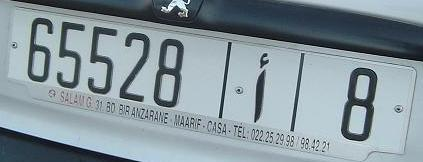
\includegraphics[width=12cm]{images/matricule.png}
		\caption{notre image positive}
		\label{fig:figure}
	\end{center}
\end{figure}

Le but de ImageNet est de former des images, de sorte que leurs images sont assez
spécifiques. Très bien, nous avons toutes ces images, et maintenant? Eh bien, enpremier lieu, nous voulons tous que tous soient de la même taille et beaucoup plus
petits! Bon sang, si seulement nous savions comment manipuler les images ... hmm ...
Ah oui, c'est un tutoriel OpenCV! Nous pouvons probablement le gérer. Donc, en premier
lieu, nous allons écrire un script rapide qui visitera ces listes d’URL, récupérera les liens,
visitera les liens, extraira les images, les redimensionnera, les sauvegardera et répétera
jusqu’à ce que nous ayons terminé. Lorsque nos répertoires sont remplis d'images, nous
avons également besoin d'une sorte de fichier de description décrivant les images. Pour
les positifs, ce fichier est une tâche difficile à créer manuellement, car vous devez
spécifier la région d'intérêt exacte de votre objet, par image. Brut. Heureusement, la
méthode createsamples place l'image de manière aléatoire et fait tout ce qui fonctionne
pour nous.


\begin{figure}[H]
	\begin{center}
		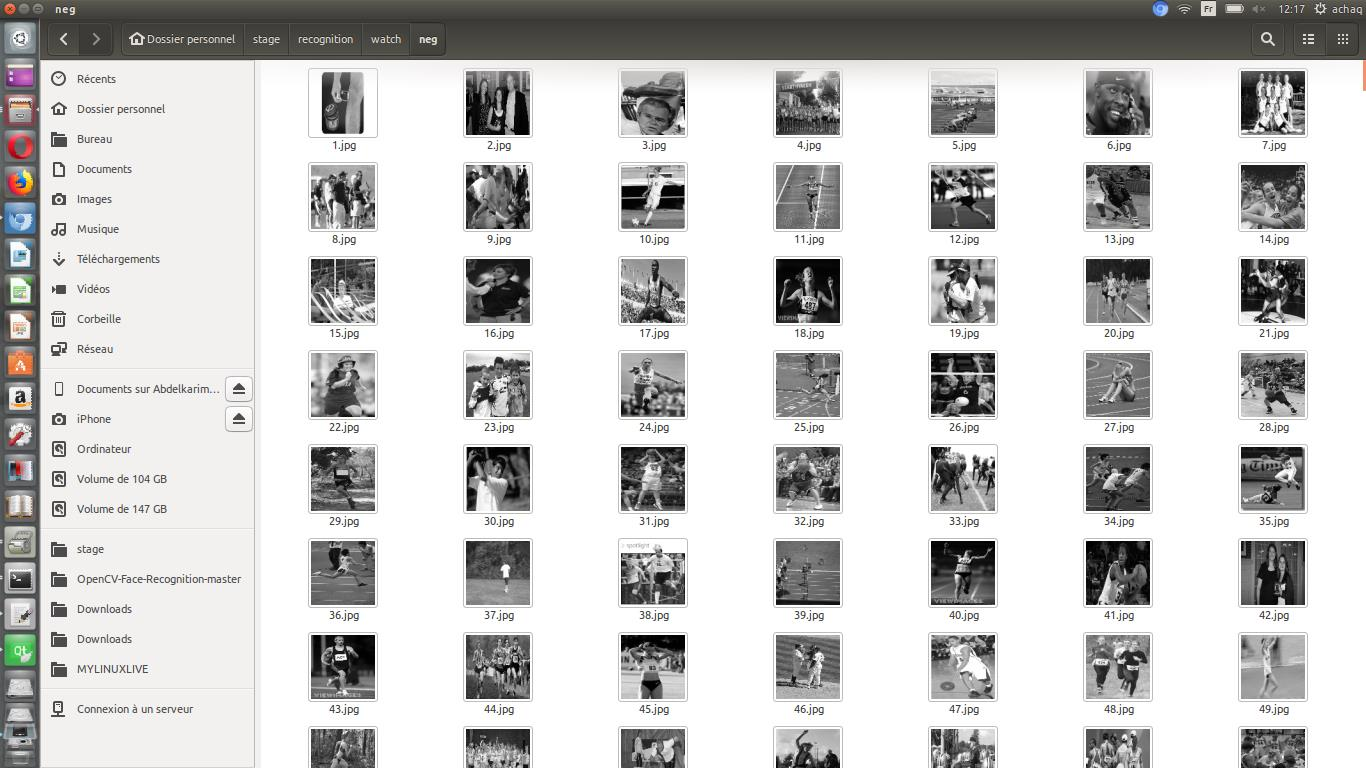
\includegraphics[width=12cm]{images/negimg.png}
		\caption{les images negatives}
		\label{fig:figure}
	\end{center}
\end{figure}

Assez simple, ce script visitera les liens, récupérera les URL et procédera à leur visite. De
là, nous prenons l'image, nous convertissons en niveaux de gris, nous la redimensionnons,
puis nous l'enregistrons. Nous utilisons un simple compteur pour nommer les
images. Allez-y et lancez-le. Comme vous pouvez probablement le voir, il y a beaucoup
d'images manquantes et autres. C'est bon. Certaines de ces images d’erreur sont plus
problématiques. Fondamentalement tout blanc avec du texte qui dit qu'ils ne sont plus disponibles, plutôt que de servir et d'erreur HTTP. Maintenant, nous avons quelques
choix. Nous pouvons simplement ignorer ceci ou le corriger. Hé, c'est une image sans
montre, alors quoi de neuf? Bien sûr, vous pouvez prendre cette opinion, mais si vous
utilisez cette méthode de tirage pour le positif, alors c'est certainement un problème. Vous
pouvez les supprimer manuellement ... ou simplement utiliser nos nouvelles
connaissances en analyse d'image pour détecter ces images stupides et les supprimer!



\begin{figure}[H]
	\begin{center}
		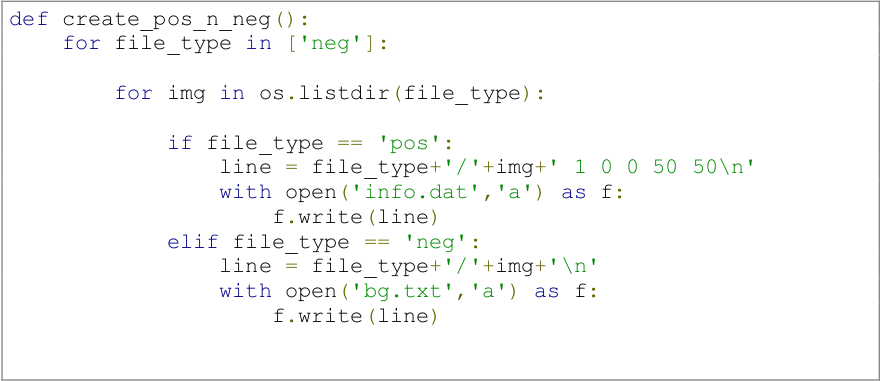
\includegraphics[width=12cm]{images/codeneg.png}
		\caption{le code pour trier les images}
		\label{fig:figure}
	\end{center}
\end{figure}

Maintenant, nous avons plus de 2 000 photos, donc nous cuisinons. La dernière étape
consiste à créer le fichier descripteur pour ces images négatives. Encore une fois, nous
allons utiliser du code!

Nous sommes prêts à créer des échantillons positifs maintenant, basés sur l’image
existante du matricule mat50x50.jpg . Pour ce faire, on va exécuter les opérations
suivantes via le terminal, alors que dans l'espace de travail

\subsection*{opencvcreatesamples -img watch5050.jpg -bg bg.txt -info
	info/info.lst -pngoutput info -maxxangle 0.5 -maxyangle 0.5 -
	maxzangle 0.5 -num 1950}


Qu'est-ce que cela fait est de créer des échantillons, basé sur l'img que nous spécifions,
bg est l'information de fond, l'information où nous allons mettre la sortie info.list (qui est
beaucoup le fichier bg.txt), alors le -pngoutput est où nous vouloir placer les images
nouvellement générées. Enfin, nous avons quelques paramètres optionnels pour rendre
notre image originale un peu plus dynamique et ensuite = num pour le nombre
d’échantillons que nous voulons essayer de créer. Super, allons faire ça. Maintenant, vous
devriez avoir ~ 2.000 images dans votre répertoire info et un fichier appelé info.lst

\begin{figure}[H]
	\begin{center}
		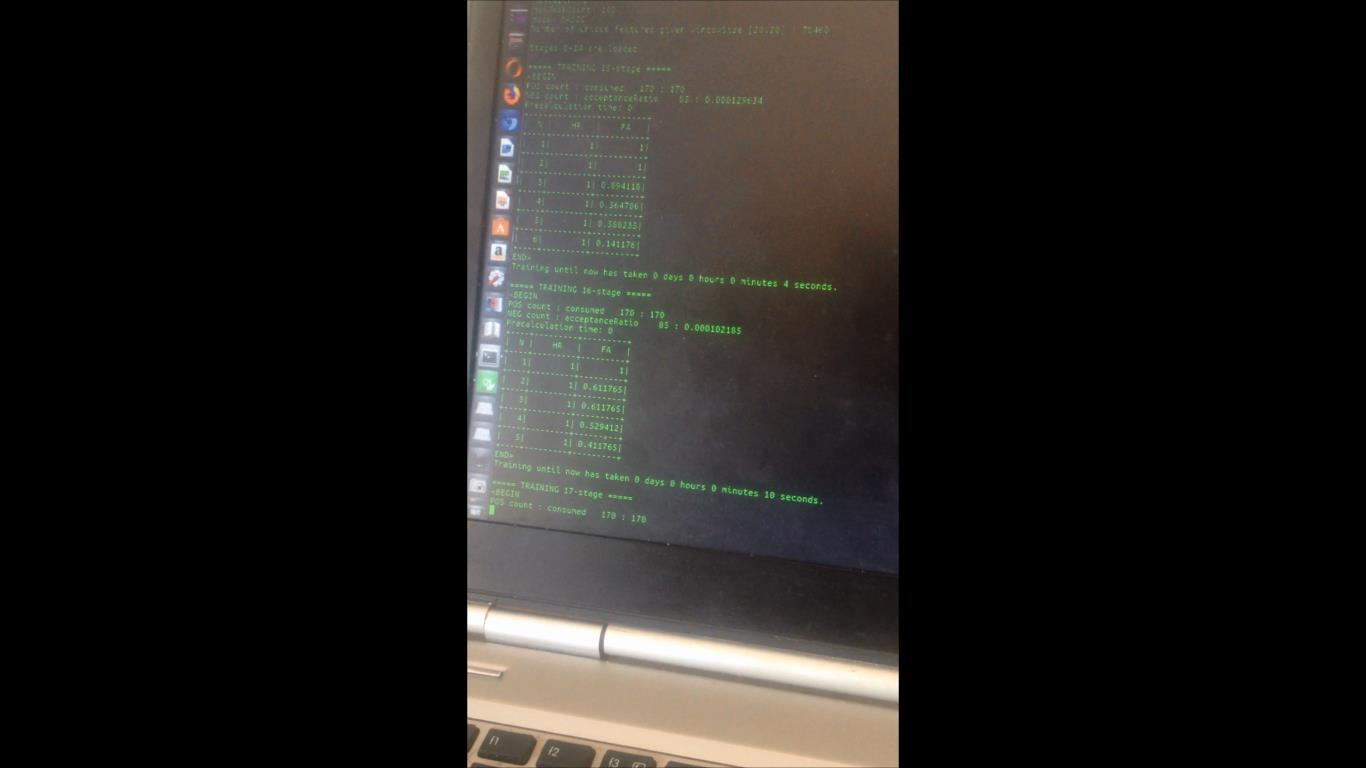
\includegraphics[width=12cm]{images/training.png}
		\caption{la phase d'entrainement}
		\label{fig:figure}
	\end{center}
\end{figure}

15 étapes ont pris un peu moins de 2 heures à faire sur mon ordinateur . Donc, soit vous
avez un fichier cascade.xml, soit vous avez arrêté l'exécution du script. Si vous l'avez
empêché de fonctionner, vous devriez avoir un tas de fichiers stageX.xml dans votre
répertoire "data". Ouvrez-le, voyez le nombre d'étapes que vous avez effectuées, puis
relancez l'opération opencvtraincascade avec ce nombre d'étapes et vous recevrez
immédiatement un fichier cascade.xml. A partir de là, j'aime juste lui donner un nom et
combien
d'étapes. Pour
moi,
j'ai
fait
10
étapes,
donc
je
le
renomme platecascade.xml. C'est tout ce dont nous avons besoin, alors retournez sur
votre ordinateur principal avec votre nouveau fichier de cascade, placez-le dans votre
répertoire de travail, et essayons!

\subsection*{resultat}
\begin{figure}[H]
	\begin{center}
		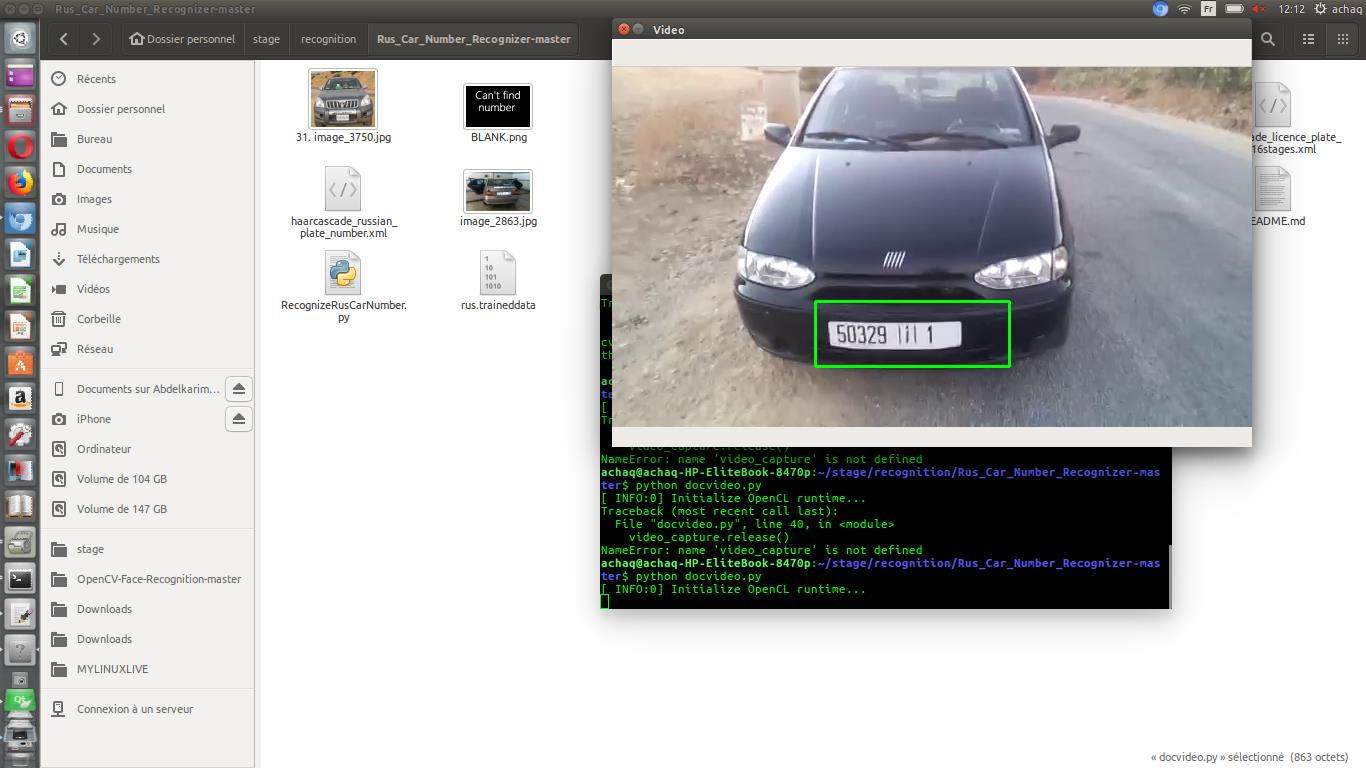
\includegraphics[width=12cm]{images/matriculedetected.png}
		\caption{le code pour trier les images}
		\label{fig:figure}
	\end{center}
\end{figure}
\section{Techniques et outils de Reconnaissance Optique des Caractères
	: en utilisant Reconnaissance des chiffres numérisés à l'aide du k-voisin le plus proche (k-NN)}
le traitement presenté ici , est fait pour les numero, le meme traitement se fait pour les characteres arabe.

\subsection{Pré-traitement de l'image}
Le script TextCleaner de Fred Weinhaus ( http://www.fmwconcepts.com/imagemagick/textcleaner/ ) a été utilisé pour supprimer le bruit de fond d’image suivi d’une étape de netteté de l’image. Ces deux étapes nécessitent la bibliothèque ImageMagick ( https://www.imagemagick.org ). Autrement, je vous recommande d'utiliser les bibliothèques de python telles que OpenCV ou scikit-image pour prétraiter les images.

\subsection{Extraction de chiffres et préparation de données}
La sélection de chaque chiffre d'une image à l'aide de l' opération findContour d'OpenCV n'a pas produit de résultats fiables en raison du bruit. Pour ce problème spécifique, il était plus robuste de détecter le «cadre de délimitation» autour des chiffres (cadrage de l'image), puis de «distinguer» chaque chiffre de l'image recadrée. Cette dernière étape est facile après avoir trouvé le cadre de sélection, car chaque chiffre aura des coordonnées fixes par rapport au coin supérieur gauche de l’image recadrée.

Remarque: les pixels noirs / blancs ont été inversés, ce qui est nécessaire pour l'extraction de caractéristiques à l'aide de l'histogramme de dégradé orienté (HOG).

\subsection{Extraction de fonctionnalités}

L'extraction de caractéristiques ou l'ingénierie de caractéristiques est le processus d'identification des caractéristiques uniques d'une entrée (chiffre dans notre cas) pour permettre à un algorithme d'apprentissage automatique (dans notre cas, de regrouper des chiffres similaires). L’ histogramme des dégradés orientés (HOG) a été utilisé avec succès dans de nombreuses applications de reconnaissance optique des caractères pour extraire du texte manuscrit. Le code suivant illustre l'extraction de HOG d'une image à l'aide de la fonction porc de skimage .

Dans mon cas, l'image fait 50 x 50 pixels et les paramètres d'entrée de hog ( pixels\_per\_cell et cells\_per\_block ) ont été définis de manière empirique. La figure ci-dessous illustre l'application de HOG sur une image produisant un vecteur de 200 valeurs (c'est-à-dire des entités).

\subsection{formation}
Au cours des étapes précédentes, nous avons extrait des chiffres similaires dans des dossiers pour construire notre jeu de données de formation. Le code ci-dessous illustre la construction de notre ensemble de données de formation 


\subsection{Prediction}

Le processus de prédiction de chiffres sur de nouvelles images suit les mêmes étapes que pour sélectionner les chiffres illustrés dans les étapes d'apprentissage ci-dessus, puis d'appliquer simplement la fonction de prédiction de k-NN 

La fonction de prédiction de k-NN renvoie une valeur à un chiffre comprise entre 0 et 9 pour désigner la classe de prédiction de l'image d'entrée. La fonction predict\_proba de K-NN renvoie la précision associée à chaque classe prédite.

Par exemple, supposons que nous ayons appliqué la prédiction sur une image contenant le chiffre «5». Un exemple de sortie serait prediction=5 and predict\_proba =[[0 0 0 0 0 .8 0 0 .2 0]] . Cela signifie que k-NN a classé l'image comme «5» avec une confiance de 80\% et comme «8» avec une confiance de 20\%.

Enfin, vous predictions = list(map(lambda x: predict(x), hogs))obtenez le vecteur de nuplets suivant, où chaque tuple représente la classe prédite de chacun des chiffres de l'image avec son assurance de prédiction associée. Toute prédiction qui ne classe pas une entrée avec une confiance de 100% sera présentée à l'utilisateur pour une correction manuelle, comme illustré dans la section suivante.

[ 
(5, 1,0), (1, 1,0), (9, 1,0), (2, 1,0), (1, 1,0), (2, 1,0), (4,1,0), (7, 1,0), ( 2, 1,0), (3, 1,0), (4, 1,0), (3, 1,0), (4, 1,0), 
(4, 0,8) , (0, 1,0) 
]

\subsection{Presentation}
\begin{figure}[H]
	\begin{center}
		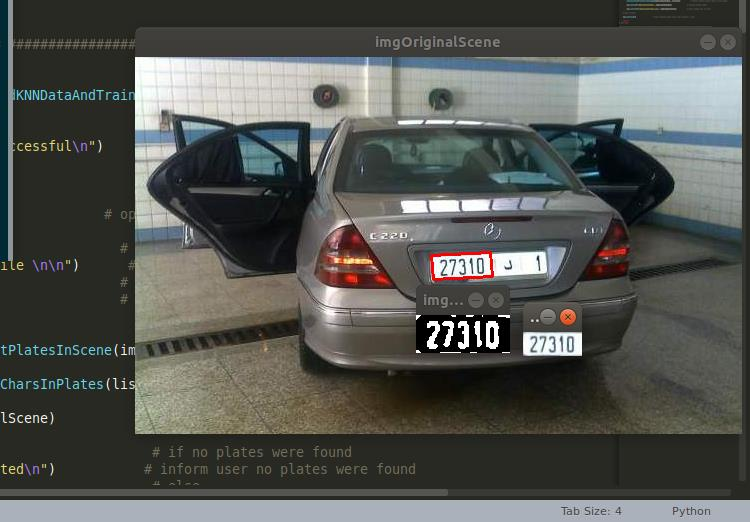
\includegraphics[width=12cm]{images/OCR.png}
		\caption{le resultat d'algorithme KNN}
		\label{fig:figure}
	\end{center}
\end{figure}

%-------------------------------------------------------------------------------------------------------------------
%
%**************************************** Detection de conteur *******************************************
%
%-------------------------------------------------------------------------------------------------------------------


%-------------------------------------------------------------------------------------------------------------------
%
%******************************************* Conclusion ************************************************
%
%-------------------------------------------------------------------------------------------------------------------
\chapter*{Conclusion}
\addcontentsline{toc}{chapter}{\numberline{}Conclusion}

\paragraph{
L’objectif de notre travail est de développer un système de détection et de
reconnaissance de plaques minéralogiques ayant la capacité d’extraire les numéros
d’immatriculation Marocaine.}
\paragraph{
Après avoir présenté un état de l’art sur les systèmes existants, nous avons
présenté notre système LAPIA : Lecture Automatique de Plaques d’Immatriculation
Marocaines où nous avons réussi à détecter avec une grande précision les chiffres formant
le matricule de du véhicule.
En plus, d’avoir atteint l’objectif final demandé, ce projet nous a été très bénéfique
car il nous a permis de maîtriser plusieurs techniques et de manipuler des outils très
complexes.
}
\paragraph{
Enfin, ce projet était une bonne occasion pour réaliser un travail très concret, avec
des objectifs clairs et bien définis et de se familiariser avec un environnement de
développement professionnel.
Comme perspectives, nous souhaiterons améliorer les résultats obtenus en
analysant les cas de défaillances et en spécifiant mieux l’OCR.
}






%-------------------------------------------------------------------------------------------------------------------
%
%**************************************** Bibliography *******************************************
%
%-------------------------------------------------------------------------------------------------------------------
\newpage

\bibliographystyle{alpha}	
\bibliography{sample}
\thispagestyle{empty}


[1]Hamid, N. A., \& Sjarif, N. N. A. (2017). Handwritten Recognition Using SVM, KNN and Neural Network. arXiv preprint arXiv:1702.00723.

[2]Adrian Rosebrock’s blogs and books (https://www.pyimagesearch.com). Great computer vision resources and many posts on digits recognition.

[3]Patel, I., Jagtap, V., \& Kale, O. (2014). A Survey on Feature Extraction Methods for Handwritten Digits Recognition. International Journal of Computer Applications, 107(12).
\newpage

\appendix

\end{document}
